\documentclass[tikz, preview]{standalone}

\usepackage{amsfonts, amsthm, amssymb, amsmath, stmaryrd, etoolbox}
\usepackage{tikz}
\usepackage[all,2cell]{xy}
\usetikzlibrary{matrix,arrows,shapes,decorations.markings,decorations.pathreplacing}
\definecolor{rewritecolor}{rgb}{0,.9,1}
\tikzset{rewritenode/.style={shape=circle,fill=rewritecolor,scale=0.25,font=\Huge}}
\tikzset{RWopen/.style={shape=circle,draw=black,fill=white,scale=0.5,font=\Huge}}
\tikzset{RWclosed/.style={shape=circle,fill=black,scale=0.5,font=\Huge}}
\tikzset{CDnode/.style={shape=circle,fill=white,scale=.5}}
\tikzset{zxgreen/.style={shape=circle,draw,thick,fill=green}}
\tikzset{zxred/.style={shape=circle,draw,thick,fill=red}}
\tikzset{zxyellow/.style={shape=rectangle,draw,thick,fill=yellow}}
\tikzset{zxdiamond/.style={shape=diamond,fill=black,inner sep=2.75}}
\tikzset{zxopen/.style={shape=circle,draw,thick,inner sep=2pt}}
\tikzset{->-/.style={decoration={markings,mark=at position .5 with {\arrow{>}}},postaction={decorate}}}

\begin{document}
\[
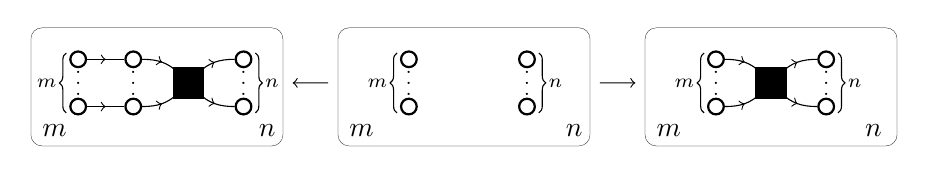
\begin{tikzpicture}
	%
	%
	%
	\begin{scope}[shift={(-1.3,0.1)}]
	\node (v1) at (0.2,-0.5) {};
	\node [zxopen] (v2) at (-0.5,-0.2) {};
	\node [zxopen] (v3) at (-0.5,-0.8) {};
	\node [zxopen] (v4) at (0.9,-0.2) {};
	\node [zxopen] (v5) at (0.9,-0.8) {};
	\node [zxopen] (v6) at (-1.2,-0.2) {};
	\node [zxopen] (v7) at (-1.2,-0.8) {};
	\node at (-0.5,-0.4) {\scriptsize $\vdots$};
	%
	\draw [->-] (v2) to [in=135,out=0] (v1);
	\draw [->-] (v3) to [in=-135,out=0] (v1);
	\draw [->-] (v1) to [in=180,out=45] (v4);
	\draw [->-] (v1) to [in=180,out=-45] (v5);
	\draw [->-] (v6) to (v2);
	\draw [->-] (v7) to (v3);
	\node at (-1.2,-0.4) {\scriptsize $\vdots$};
	\node at (0.9,-0.4) {\scriptsize $\vdots$};
	%
	\node (v8) at (0.4,-0.7) {};
	\node (v9) at (0,-0.3) {};
	\fill [black] (v8) rectangle (v9);
	%
	\draw[decoration={brace,mirror,raise=2pt},decorate]
	(v6.north west) -- node [left=2pt] {\scriptsize $m$} (v7.south west); 
	\draw[decoration={brace,raise=2pt},decorate]
	(v4.north east) -- node [right=2pt] {\scriptsize $n$} (v5.south east); 
	%
	\node at (-1.5,-1.1) {$m$};
	\node at (1.2,-1.1) {$n$};
	\node (v11) at (1.4,-0.5) {};
	\draw [ultra thin, rounded corners] (-1.8,0.2) rectangle (1.4,-1.3);
	\end{scope}
	%
	%
	%
	\begin{scope}[shift={(3.8,-0.1)}]
	\node [zxopen] (v1) at (-2.1,0) {};
	\node [zxopen] (v2) at (-0.6,0) {};
	\node [zxopen] (v3) at (-2.1,-0.6) {};
	\node [zxopen] (v4) at (-0.6,-0.6) {};
	\node at (-2.1,-0.2) {\scriptsize $\vdots$};
	\node at (-0.6,-0.2) {\scriptsize $\vdots$};
	%
	\draw [ultra thin, rounded corners] (-3,0.4) rectangle (0.2,-1.1);
	\draw[decoration={brace,mirror,raise=2pt},decorate]
	(v1.north west) -- node [left=2pt] {\scriptsize $m$} (v3.south west);
	\draw[decoration={brace,raise=2pt},decorate]
	(v2.north east) -- node [right=2pt] {\scriptsize $n$} (v4.south east); 
	\node at (-2.7,-0.9) {$m$};
	\node at (0,-0.9) {$n$};
	\node (v12) at (-3,-0.3) {};
	\node (v14) at (0.2,-0.3) {};
	\end{scope}
	%
	%
	%
	\begin{scope}[shift={(6.7,0)}]
	\node (v1) at (-0.4,-0.4) {};
	\node [zxopen] (v2) at (-1.1,-0.1) {};
	\node [zxopen] (v3) at (-1.1,-0.7) {};
	\node [zxopen] (v4) at (0.3,-0.1) {};
	\node [zxopen] (v5) at (0.3,-0.7) {};
	%
	\draw [->-] (v2) to [in=135,out=0] (v1);
	\draw [->-] (v3) to [in=-135,out=0] (v1);
	\draw [->-] (v1) to [in=180,out=45] (v4);
	\draw [->-] (v1) to [in=180,out=-45] (v5);
	\node at (-1.1,-0.3) {\scriptsize $\vdots$};
	\node at (0.3,-0.3) {\scriptsize $\vdots$};
	%
	\node (v8) at (-0.2,-0.6) {};
	\node (v9) at (-0.6,-0.2) {};
	\fill [black] (v8) rectangle (v9);
	%
	\draw[decoration={brace,mirror,raise=2pt},decorate]
	(v2.north west) -- node [left=2pt] {\scriptsize $m$} (v3.south west); 
	\draw[decoration={brace,raise=2pt},decorate]
	(v4.north east) -- node [right=2pt] {\scriptsize $n$} (v5.south east); 
	%
	\node at (-1.7,-1) {$m$};
	\node at (0.9,-1) {$n$};
	\draw [ultra thin, rounded corners] (-2,0.3) rectangle (1.2,-1.2);
	\node (v13) at (-2,-0.4) {};
	\end{scope}
	%
	%
	%
	\draw [<-] (v11) edge (v12);
	\draw [<-] (v13) edge (v14);
\end{tikzpicture}
\]
\end{document}
